

\tikzset{every picture/.style={line width=0.75pt}} %set default line width to 0.75pt        

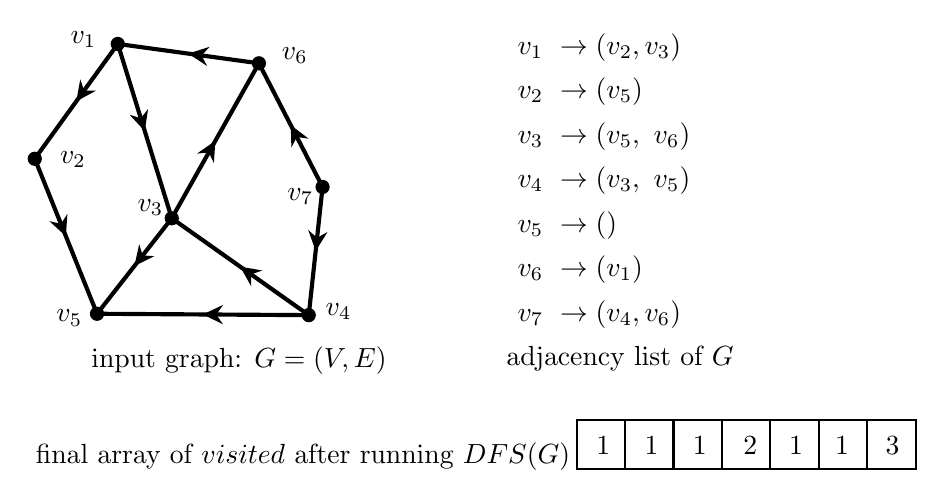
\begin{tikzpicture}[x=0.5pt,y=0.5pt,yscale=-1,xscale=1]
%uncomment if require: \path (0,342); %set diagram left start at 0, and has height of 342

%Flowchart: Connector [id:dp9968125919431555] 
\draw  [fill={rgb, 255:red, 0; green, 0; blue, 0 }  ,fill opacity=1 ] (78,14) .. controls (78,11.58) and (79.96,9.62) .. (82.38,9.62) .. controls (84.79,9.62) and (86.75,11.58) .. (86.75,14) .. controls (86.75,16.42) and (84.79,18.38) .. (82.38,18.38) .. controls (79.96,18.38) and (78,16.42) .. (78,14) -- cycle ;
%Flowchart: Connector [id:dp31888007270335605] 
\draw  [fill={rgb, 255:red, 0; green, 0; blue, 0 }  ,fill opacity=1 ] (180,28) .. controls (180,25.58) and (181.96,23.62) .. (184.38,23.62) .. controls (186.79,23.62) and (188.75,25.58) .. (188.75,28) .. controls (188.75,30.42) and (186.79,32.38) .. (184.38,32.38) .. controls (181.96,32.38) and (180,30.42) .. (180,28) -- cycle ;
%Flowchart: Connector [id:dp7333018163719219] 
\draw  [fill={rgb, 255:red, 0; green, 0; blue, 0 }  ,fill opacity=1 ] (63,209) .. controls (63,206.58) and (64.96,204.62) .. (67.38,204.62) .. controls (69.79,204.62) and (71.75,206.58) .. (71.75,209) .. controls (71.75,211.42) and (69.79,213.38) .. (67.38,213.38) .. controls (64.96,213.38) and (63,211.42) .. (63,209) -- cycle ;
%Flowchart: Connector [id:dp3353783499113435] 
\draw  [fill={rgb, 255:red, 0; green, 0; blue, 0 }  ,fill opacity=1 ] (18,97) .. controls (18,94.58) and (19.96,92.62) .. (22.38,92.62) .. controls (24.79,92.62) and (26.75,94.58) .. (26.75,97) .. controls (26.75,99.42) and (24.79,101.38) .. (22.38,101.38) .. controls (19.96,101.38) and (18,99.42) .. (18,97) -- cycle ;
%Flowchart: Connector [id:dp041293046821785806] 
\draw  [fill={rgb, 255:red, 0; green, 0; blue, 0 }  ,fill opacity=1 ] (117,140) .. controls (117,137.58) and (118.96,135.62) .. (121.38,135.62) .. controls (123.79,135.62) and (125.75,137.58) .. (125.75,140) .. controls (125.75,142.42) and (123.79,144.38) .. (121.38,144.38) .. controls (118.96,144.38) and (117,142.42) .. (117,140) -- cycle ;
%Straight Lines [id:da670830947000866] 
\draw [color={rgb, 255:red, 0; green, 0; blue, 0 }  ,draw opacity=1 ][line width=1.5]    (22.38,97) -- (82.38,14) ;
\draw [shift={(52.38,55.5)}, rotate = 305.86] [fill={rgb, 255:red, 0; green, 0; blue, 0 }  ,fill opacity=1 ][line width=0.08]  [draw opacity=0] (14.56,-6.99) -- (0,0) -- (14.56,6.99) -- (9.67,0) -- cycle    ;
%Straight Lines [id:da11972331039419015] 
\draw [color={rgb, 255:red, 0; green, 0; blue, 0 }  ,draw opacity=1 ][line width=1.5]    (67.38,209) -- (121.38,140) ;
\draw [shift={(94.38,174.5)}, rotate = 308.05] [fill={rgb, 255:red, 0; green, 0; blue, 0 }  ,fill opacity=1 ][line width=0.08]  [draw opacity=0] (14.56,-6.99) -- (0,0) -- (14.56,6.99) -- (9.67,0) -- cycle    ;
%Straight Lines [id:da5479420807598677] 
\draw [color={rgb, 255:red, 0; green, 0; blue, 0 }  ,draw opacity=1 ][line width=1.5]    (121.38,140) -- (82.38,14) ;
\draw [shift={(101.88,77)}, rotate = 252.8] [fill={rgb, 255:red, 0; green, 0; blue, 0 }  ,fill opacity=1 ][line width=0.08]  [draw opacity=0] (14.56,-6.99) -- (0,0) -- (14.56,6.99) -- (9.67,0) -- cycle    ;
%Straight Lines [id:da5035840510752034] 
\draw [color={rgb, 255:red, 0; green, 0; blue, 0 }  ,draw opacity=1 ][line width=1.5]    (67.38,209) -- (22.38,97) ;
\draw [shift={(44.88,153)}, rotate = 248.11] [fill={rgb, 255:red, 0; green, 0; blue, 0 }  ,fill opacity=1 ][line width=0.08]  [draw opacity=0] (14.56,-6.99) -- (0,0) -- (14.56,6.99) -- (9.67,0) -- cycle    ;
%Flowchart: Connector [id:dp2827777113276231] 
\draw  [fill={rgb, 255:red, 0; green, 0; blue, 0 }  ,fill opacity=1 ] (216,210) .. controls (216,207.58) and (217.96,205.62) .. (220.38,205.62) .. controls (222.79,205.62) and (224.75,207.58) .. (224.75,210) .. controls (224.75,212.42) and (222.79,214.38) .. (220.38,214.38) .. controls (217.96,214.38) and (216,212.42) .. (216,210) -- cycle ;
%Straight Lines [id:da4794154088615755] 
\draw [color={rgb, 255:red, 0; green, 0; blue, 0 }  ,draw opacity=1 ][line width=1.5]    (220.38,210) -- (121.38,140) ;
\draw [shift={(170.88,175)}, rotate = 35.26] [fill={rgb, 255:red, 0; green, 0; blue, 0 }  ,fill opacity=1 ][line width=0.08]  [draw opacity=0] (14.56,-6.99) -- (0,0) -- (14.56,6.99) -- (9.67,0) -- cycle    ;
%Straight Lines [id:da5289435706939755] 
\draw [color={rgb, 255:red, 0; green, 0; blue, 0 }  ,draw opacity=1 ][line width=1.5]    (67.38,209) -- (220.38,210) ;
\draw [shift={(143.88,209.5)}, rotate = 0.37] [fill={rgb, 255:red, 0; green, 0; blue, 0 }  ,fill opacity=1 ][line width=0.08]  [draw opacity=0] (14.56,-6.99) -- (0,0) -- (14.56,6.99) -- (9.67,0) -- cycle    ;
%Flowchart: Connector [id:dp11045273073359585] 
\draw  [fill={rgb, 255:red, 0; green, 0; blue, 0 }  ,fill opacity=1 ] (226,117.38) .. controls (226,114.96) and (227.96,113) .. (230.38,113) .. controls (232.79,113) and (234.75,114.96) .. (234.75,117.38) .. controls (234.75,119.79) and (232.79,121.75) .. (230.38,121.75) .. controls (227.96,121.75) and (226,119.79) .. (226,117.38) -- cycle ;
%Straight Lines [id:da34875485243986093] 
\draw [color={rgb, 255:red, 0; green, 0; blue, 0 }  ,draw opacity=1 ][line width=1.5]    (230.38,117.38) -- (184.38,28) ;
\draw [shift={(207.38,72.69)}, rotate = 62.77] [fill={rgb, 255:red, 0; green, 0; blue, 0 }  ,fill opacity=1 ][line width=0.08]  [draw opacity=0] (14.56,-6.99) -- (0,0) -- (14.56,6.99) -- (9.67,0) -- cycle    ;
%Shape: Grid [id:dp773013244810068] 
\draw  [draw opacity=0] (414,285.87) -- (659,285.87) -- (659,320.87) -- (414,320.87) -- cycle ; \draw   (449,285.87) -- (449,320.87)(484,285.87) -- (484,320.87)(519,285.87) -- (519,320.87)(554,285.87) -- (554,320.87)(589,285.87) -- (589,320.87)(624,285.87) -- (624,320.87) ; \draw    ; \draw   (414,285.87) -- (659,285.87) -- (659,320.87) -- (414,320.87) -- cycle ;
%Straight Lines [id:da6438487476256122] 
\draw [color={rgb, 255:red, 0; green, 0; blue, 0 }  ,draw opacity=1 ][line width=1.5]    (121.38,140) -- (184.38,28) ;
\draw [shift={(152.88,84)}, rotate = 119.36] [fill={rgb, 255:red, 0; green, 0; blue, 0 }  ,fill opacity=1 ][line width=0.08]  [draw opacity=0] (14.56,-6.99) -- (0,0) -- (14.56,6.99) -- (9.67,0) -- cycle    ;
%Straight Lines [id:da22153267574847257] 
\draw [color={rgb, 255:red, 0; green, 0; blue, 0 }  ,draw opacity=1 ][line width=1.5]    (82.38,14) -- (184.38,28) ;
\draw [shift={(133.38,21)}, rotate = 7.82] [fill={rgb, 255:red, 0; green, 0; blue, 0 }  ,fill opacity=1 ][line width=0.08]  [draw opacity=0] (14.56,-6.99) -- (0,0) -- (14.56,6.99) -- (9.67,0) -- cycle    ;
%Straight Lines [id:da1089086337589269] 
\draw [color={rgb, 255:red, 0; green, 0; blue, 0 }  ,draw opacity=1 ][line width=1.5]    (220.38,210) -- (230.38,117.38) ;
\draw [shift={(225.38,163.69)}, rotate = 276.16] [fill={rgb, 255:red, 0; green, 0; blue, 0 }  ,fill opacity=1 ][line width=0.08]  [draw opacity=0] (14.56,-6.99) -- (0,0) -- (14.56,6.99) -- (9.67,0) -- cycle    ;

% Text Node
\draw (46,3) node [anchor=north west][inner sep=0.75pt]   [align=left] {$\displaystyle v_{1}$};
% Text Node
\draw (94.38,124.38) node [anchor=north west][inner sep=0.75pt]   [align=left] {$\displaystyle v_{3}$};
% Text Node
\draw (35.75,204) node [anchor=north west][inner sep=0.75pt]   [align=left] {$\displaystyle v_{5}$};
% Text Node
\draw (230.38,199.38) node [anchor=north west][inner sep=0.75pt]   [align=left] {$\displaystyle v_{4}$};
% Text Node
\draw (38.38,89.38) node [anchor=north west][inner sep=0.75pt]   [align=left] {$\displaystyle v_{2}$};
% Text Node
\draw (369,4.09) node [anchor=north west][inner sep=0.75pt]   [align=left] {$\displaystyle v_{1} \ \rightarrow ( v_{2} ,v_{3})$};
% Text Node
\draw (369,36.26) node [anchor=north west][inner sep=0.75pt]   [align=left] {$\displaystyle v_{2} \ \rightarrow ( v_{5})$};
% Text Node
\draw (369,68.43) node [anchor=north west][inner sep=0.75pt]   [align=left] {$\displaystyle v_{3} \ \rightarrow ( v_{5} ,\ v_{6})$};
% Text Node
\draw (369,100.6) node [anchor=north west][inner sep=0.75pt]   [align=left] {$\displaystyle v_{4} \ \rightarrow ( v_{3} ,\ v_{5})$ \ };
% Text Node
\draw (369,132.77) node [anchor=north west][inner sep=0.75pt]   [align=left] {$\displaystyle v_{5} \ \rightarrow ()$};
% Text Node
\draw (198.75,14.35) node [anchor=north west][inner sep=0.75pt]   [align=left] {$\displaystyle v_{6}$};
% Text Node
\draw (202.75,116.35) node [anchor=north west][inner sep=0.75pt]   [align=left] {$\displaystyle v_{7}$};
% Text Node
\draw (369,164.94) node [anchor=north west][inner sep=0.75pt]   [align=left] {$\displaystyle v_{6} \ \rightarrow ( v_{1} )$ \ };
% Text Node
\draw (369,197.09) node [anchor=north west][inner sep=0.75pt]   [align=left] {$\displaystyle v_{7} \ \rightarrow ( v_{4} ,v_{6})$};
% Text Node
\draw (61,230.93) node [anchor=north west][inner sep=0.75pt]   [align=left] {input graph: $\displaystyle G=( V,E)$};
% Text Node
\draw (361,229.93) node [anchor=north west][inner sep=0.75pt]   [align=left] {adjacency list of $\displaystyle G$};
% Text Node
\draw (21,299.93) node [anchor=north west][inner sep=0.75pt]   [align=left] {final array of $\displaystyle visited$ after running $\displaystyle DFS( G)$};
% Text Node
\draw (426,295.37) node [anchor=north west][inner sep=0.75pt]   [align=left] {$\displaystyle 1$};
% Text Node
\draw (460.83,295.37) node [anchor=north west][inner sep=0.75pt]   [align=left] {$\displaystyle 1$};
% Text Node
\draw (495.66,295.37) node [anchor=north west][inner sep=0.75pt]   [align=left] {$\displaystyle 1$};
% Text Node
\draw (598.49,295.37) node [anchor=north west][inner sep=0.75pt]   [align=left] {$\displaystyle 1$};
% Text Node
\draw (565.32,295.37) node [anchor=north west][inner sep=0.75pt]   [align=left] {$\displaystyle 1$};
% Text Node
\draw (532.15,295.37) node [anchor=north west][inner sep=0.75pt]   [align=left] {$\displaystyle 2$};
% Text Node
\draw (635,295.37) node [anchor=north west][inner sep=0.75pt]   [align=left] {$\displaystyle 3$};


\end{tikzpicture}

